
\documentclass[10pt, conference, letterpaper]{IEEEtran}

\usepackage{comment}
\usepackage{amsthm}
\usepackage{amssymb}
\usepackage{amsmath}
\interdisplaylinepenalty=2500
\usepackage{graphicx}
\graphicspath{{figs/}}
\usepackage[font=small]{caption}
\usepackage[labelformat=simple,font=scriptsize]{subcaption}
\renewcommand\thesubfigure{(\alph{subfigure})}

\usepackage[dvipsnames]{xcolor}
\usepackage{cite}
\usepackage{hyperref}
\usepackage{algorithm}
\usepackage{algorithmic}
\usepackage{lastpage}
\usepackage{setspace}
\usepackage{adjustbox}

\newcommand{\etal}{\textit{et~al.}}
\newcommand{\eg}{\textit{e.g.},}
\newcommand{\ie}{\textit{i.e.},}
\newcommand{\etc}{\textit{etc}.\@}
\newcommand{\eqend}{\,.}

\newcommand{\mg}[1]{{\color{Red}[MG]} {\color{Blue}#1} }
\newcommand{\highlight}[1]{{\color{Red}#1}}
\newcommand{\cat}[1]{\medskip\noindent\textbf{#1.}}
\newcommand{\fcat}[1]{\noindent\textbf{#1.}}

\newcommand{\pr}[1]{\mathbb{P}\left\{#1\right\}}
\newcommand{\E}[1]{\mathbb{E}\left[#1\right]}
\newcommand{\V}[1]{\mathrm{Var}\left(#1\right)}
\newcommand{\ol}[1]{\overline{#1}}
\newcommand{\mx}[1]{\ensuremath{\mathbf{#1}}}
\newcommand{\mc}[1]{\mathcal{#1}}
\newcommand{\set}[1]{\left\{ #1 \right\}}
\newcommand{\ang}[1]{\langle #1 \rangle}



\newbox\bwk\edef\tempd#1pt{#1\string p\string t}\tempd\def\nbextr#1pt{#1}
\def\npts#1{\expandafter\nbextr\the#1\space}
\def\ttwplink#1#2{\special{ps:1 0 0 setrgbcolor}#2\special{ps:0 0 0 setrgbcolor}\setbox\bwk=\hbox{#2}\special{ps:( linkto #1)\space\npts{\wd\bwk} \npts{\dp\bwk} -\npts{\ht\bwk} true\space Cpos}}
\begin{document}

\title{A GAN-based Covert Channel over Autoencoder Wireless Communication Systems}

\author{
	\IEEEauthorblockN{Ali Mohammadi Teshnizi}
	\IEEEauthorblockA{Dept. Computer Science\\
		University of Calgary\\
		{ali.mohammaditeshniz@ucalgary.ca}}
	\and
	\IEEEauthorblockN{Majid Ghaderi}
	\IEEEauthorblockA{Dept. Computer Science\\ 
		University of Calgary\\
		{mghaderi@ucalgary.ca}}
	\and	
	\IEEEauthorblockN{ Dennis Goeckel}
	\IEEEauthorblockA{Dept. Electrical and Computer Engineering\\ 
		University of Massachusetts Amherst\\
		{goeckel@ecs.umass.edu}}
}

\maketitle
\begin{abstract}
Hiding the wireless communication by transmitter Alice to intended receiver Bob from a capable and attentive adversary Willie has been widely studied under the moniker ``covert communications''.  However, when such covert communication is done in the presence of allowable system communications, there has been little study of both hiding the signal and preserving the performance of those allowable communications. Here, by treating Alice, Bob, and Willie as a generator, decoder, and discriminator neural network, we perform joint training in an adversarial setting to yield a covert communication scheme that can be added to any normal autoencoder. The method does not depend on the characteristics of the cover signal or the type of channel and it is developed for both single-user and multi-user systems. Numerical results indicate that we are able to establish a reliable undetectable channel between Alice and Bob, regardless of the cover signal or type of fading, and that the signal causes almost no disturbance to the ongoing normal operation of the system.
\end{abstract}

\begin{comment}
	Covert communication, wireless communication, autoencoder wireless systems
\end{comment}
\section{Introduction}
\label{s:intro}

Due to the shared and broadcast nature of wireless channels, there is considerable attention on the security and privacy aspects of wireless communications. While traditional cryptography methods and physical-layer securities can protect the confidentiality of the content (i.e the information transmitted over the channel), there are occasions that hiding the very existence of the communication channel is more vital than securing the communicated message itself. Examples of such situations are military operations, cyber-espionage, social unrest, or communication parties' privacy. All above have motivated the study of hidden communication channels, namely, "covert channels" \cite{lampson1973note}.\\
The preliminary attempt to obtain covertness started with the study of spread spectrum, which began almost a century ago with the main purpose of hiding military communications. The idea is to spread the transmit power into the noise so that the communication stays hidden. Many works continued to further examine different aspects of this idea, yet the fundamental performance limits of such work were unknown until recently when Bash et al. \cite{bash2012square} established a square root limit on the number of covert bits that can be reliably sent over an additive white Gaussian noise (AWGN) channel while remaining covert to a channel's observer. Followed by this work, there has been a surge of interest in examining covert channels \cite{sobers2017covert,soltani2018covert} especially in point-to-point wireless communication models.\\
In the last decade, majority of the research works on covert communication focus on integration of covert communication techniques into the current and future wireless technologies, such as 6G wireless networks and IoT. With the advent of AI and recent advances in computer's computation power and algorithmic designs, machine learning (ML) is now becoming an integral part of many research topics. Correspondingly, wireless community started to adopt machine learning techniques and use them as solutions to the various network optimization problems, which were traditionally handled with statistical models. Deep neural networks (DNNs) in particular, a major force in machine learning, are now applied into many of these tasks including signal classification, channel estimation, transmitter identification, jamming and anti-jamming [?].\\
More recently, as a replacement for conventional modular-based designs, an end-to-end communication model based on deep learning methods has emerged \cite{o2017introduction}. In this new paradigm, the transmitter and receiver are jointly trained as the encoder and decoder of an autoencoder network. While the transmitter learns to encode the transmitted symbol to an embedding vector of wireless signals, the decoder, on the other side, learns to retrieve that symbol back from the transmitted signal after passing through the channel. One noticeable difference between end-to-end systems and conventional modular designs is that in end-to-end systems, the encoder learns coding and modulation tasks simultaneously as opposed to having separate modules to perform each task. This is also true for the decoder of the system that jointly learns demodulation and decoding. Given the fact that channel distortions usually have a non-linear behavior, a DNN-based communication model is expected to capture these dissimilitudes better compared to a statistical model. That means, these systems can learn more complex channel effects and can operate more robustly under different noise levels and channel imperfections \cite{wang2017deep}.
In this work, we introduce a novel deep learning based covert communication method inspired by steganography techniques using generative adversarial networks (GANs). The proposed covert scheme is designed for the next generation autoencoder-based wireless communication models, which are believed to be replacing traditional modular based wireless systems in the near future. However, there is no limitation on integrating our covert model to the current wireless communication systems.\\
The contributions of this work can be expressed as:
\begin{enumerate}
	\item We propose a novel covert communication method using GANs that works independent of the channel and cover signals of the wireless system.
	\item We train and evaluate our system on two different channel models of AWGN and Rayleigh fading to be more compliant to a realistic wireless communication model.
	\item We also measured both the performance of our covert model and the normal autoencoder-based communication system in terms of error rates to comprehend effectiveness of covert scheme and the impact of it on the existing communication between normal users.
\end{enumerate}

\section{Related Works}
\label{s:related}
Since the main idea of our work stems from the stenography techniques, we first briefly go over the history and the current state of this field of research. We then continue this section reviewing some of the existing approaches of establishing covert communication at the physical layer of wireless networks.


\textbf{Image Steganography}: Deep learning algorithms have proven their efficiency in many aspects. Steganography is one of these areas that has benefited tremendously from deep learning advancements in recent years. Convolution neural networks (CNNs) for instance, which are generally used in computer vision tasks, have shown outstanding results in image steganalysis \cite{tan2014stacked,qian2015deep,xu2016structural}, replacing the traditional statistical methods. One of the earliest works of image steganography using deep neural networks is a work by \cite{baluja2017hiding}. In this work, Baluja proposes a hiding scheme in which the three networks of preparation, hiding, and reveal sort out the secret encoding and decoding task. The preparation network transforms the hidden message into features that are commonly used for compressing images. Then, the hiding network embeds it into the cover image and sends it to the reveal network, where the secret message gets extracted from the container image. Following this work, it was discovered that the existence of preparation network is not necessary and the framework can be expressed in a simpler form by excluding this network \cite{zhang2021brief}. The disadvantage of these schemes is that the encoding process is reliant on the cover image. To address this, Zhang et al. \cite{zhang2020udh} propose a new architecture in which secret message can be encoded independent of the cover image. Beside having more flexibility on hiding the information, this approach has also become an effective method for image watermarking. To manifest robustness against steganalysis practices, researchers started to adopt generative adversarial network (GAN) architectures \cite{goodfellow2014generative}. Volkhonskiy et al. \cite{volkhonskiy2020steganographic} propose one of the first steganography techniques based on GAN networks. The main idea of their work is to use a generative network to produce a new set of cover images that when carries the secret message using any of the available steganography techniques will be less exposed to be detected by a discriminator network (i.e. a steganalysis network). Similarly, Hayes et al. \cite{hayes2017generating} introduce a GAN-based steganography technique with a different objective for the generator network. Instead of generating cover images, the generator learns to embed secret messages into the cover images so that the discriminator cannot distinguish cover images from stenographic images. Although this adversarial scenario was preliminary introduced for hiding data in images, researchers found it so versatile that it has been applied into the other forms of data such as video, audio and text. This has inspired us to investigate the applicability of such techniques in wireless signals domain.


\textbf{Covert Communication}: Covert communication has been applied to almost every network layer and protocol, such as IP \cite{cabuk2004ip}, MAC \cite{sheikholeslami2020covert}, and DNS \cite{nussbaum2009robust}. However, covert communication at the physical layer has not been receiving much attention until recently. Dutta et al. \cite{dutta2012secret} are on of the first researchers who developed a covert communication technique for the physical layer of the wireless communication systems. They leverage the communication noise, which can be caused either by the channel or the hardware imperfections, as a mean to establish the covert channel. In their method, messages are covertly encoded in the constellation error of the normal cover signals. Similarly, Cao et al. \cite{cao2018wireless} further improved this method with the goal of reducing probability of detection. However, distortions that these methods cause in the statistical properties of the system were later found not so difficult to be detected using steganalysis methods \cite{huang2020exploiting}, which in turn results in compromising the channel. More recent works have explored the viability of deep neural networks in covert communication problem. Sankhe et al. \cite{sankhe2019impairment} propose a method called Impairment Shift Keying that produces subtle variations in normal signals in a controlled way such that a CNN model can be trained to classify them as zeros or ones. Although the impact of their covert method on the system's communication error rate is as small as 1\%,  authors in \cite{huang2021detection} showed that even tiny modifications to the signals' constellation points can be detected using a CNN model trained on the amplitude and phase characteristics of the error vector magnitude (EVM) and constellation points. Besides, their scheme relies on existing hardware impairments in the system, which is not the case in many deployments. To find an optimal solution for the highest covert rate and minimum probability of detection, Liao et al. \cite{liao2020generative} employed a GAN model that can adaptively adjust the signal power at a relay station for establishing a covert communication. This requires the covert users to have access to a cooperative relay node that is not the case in many communication scenarios. Another example of adversarial training for covert communication can be found in \cite{kim2022covert}. Their setup contains a transmitter communicating with a receiver through a Reconfigurable Intelligent Surface (RIS), and their goal is to keep this communication covert from a prospective eavesdropper. Both the intended receiver and the eavesdropper use CNN classifiers to detect the signals. This scenario raises the same concern of the previous work's that is the necessity of existence of a relay node in the deployment. Moreover, perturbations added to the signals to deceive the eavesdropper are crafted using fast gradient method (FGM) \cite{goodfellow2014explaining}, which in \cite{bahramali2021robust} was shown easy to counter using the existing countermeasure techniques. Our work differs from these two works in two aspects. First, our proposed method relies on no external entities or external factors, such as relay nodes and hardware impairments, and this helps with the generality of our model. Second, we use a generative network to produce a set of perturbations to maximize the robustness of our attacks against the system's observer or eavesdropper. 

One of the most related works to ours is the covert scheme proposed by Mohammed et al. \cite{mohammed2021adversarial}. They formulate the covert communication as a three-player game in which networks compete in an adversarial setting to obtain the optimal solution. In their setup, the encoder and decoder networks learn to covertly communicate through a form of noise and simultaneously try to confuse a detector network that tries to tell whether the users are covertly communicating or it is just the normal transmissions going through. While our proposed method shares some of the ideas of aforementioned work, there are a couple of limitations in this work that ours aims to address. First, our model is not leveraging on any hardware impairment noise and embeds the covert signals into the existing channel's noise. Second, in the previous work, the impact of added covert signals on communication is unknown, but our model is optimized to preserve the performance of normal communication. And finally, previous work assumes the channel between users to be AWGN, however, this is not an accurate model for simulating the channel effects in wireless communications due to fading. Our work addresses this by proposing a robust method against different channel models including Rayleigh and Rician fading channels.
\section{Background On Autoencoder Communication Systems}
\label{s:design}
An autoencoder-based communication system is an end-to-end learning paradigm that abstracts out the coding and modulation components of a  traditional modular communication system by replacing the transmitter and receiver with DNNs. You can see a block diagram of such a system in figure ?. The encoder (transmitter) first uses a mapping to transform \(k\) bits of data into a message \(s\) where \(s \in \{1,...,M\}\) and \(M = 2^k\). Then it takes this transformed message as an input and generates a signal \(x = E(s) \in \mathbb{R}^{2n}\), which is a real valued vector. This \(2 \times n\) dimensional real valued vector can be treated as an \(n\) dimensional complex vector where \(n\) is the number of channel uses the signal needs to be transmitted over. Then, the channel effect \(z\), which is usually considered to be AWGN, is added to the signal vector. Thus, the received signal at the receiver carries within iselfs noise of the channel and can be expressed as \(y = x + z\). The decoder (receiver) applies the transformation \(g: \mathbb{R}^{2n} \rightarrow M \) to outputs the reconstructed version of the message \(s\), which is denoted as \(\hat{s} = g(y)\).
\input{tex/model-s}
\begin{figure*}[tp!]
	\begin{subfigure}{0.3\textwidth}
		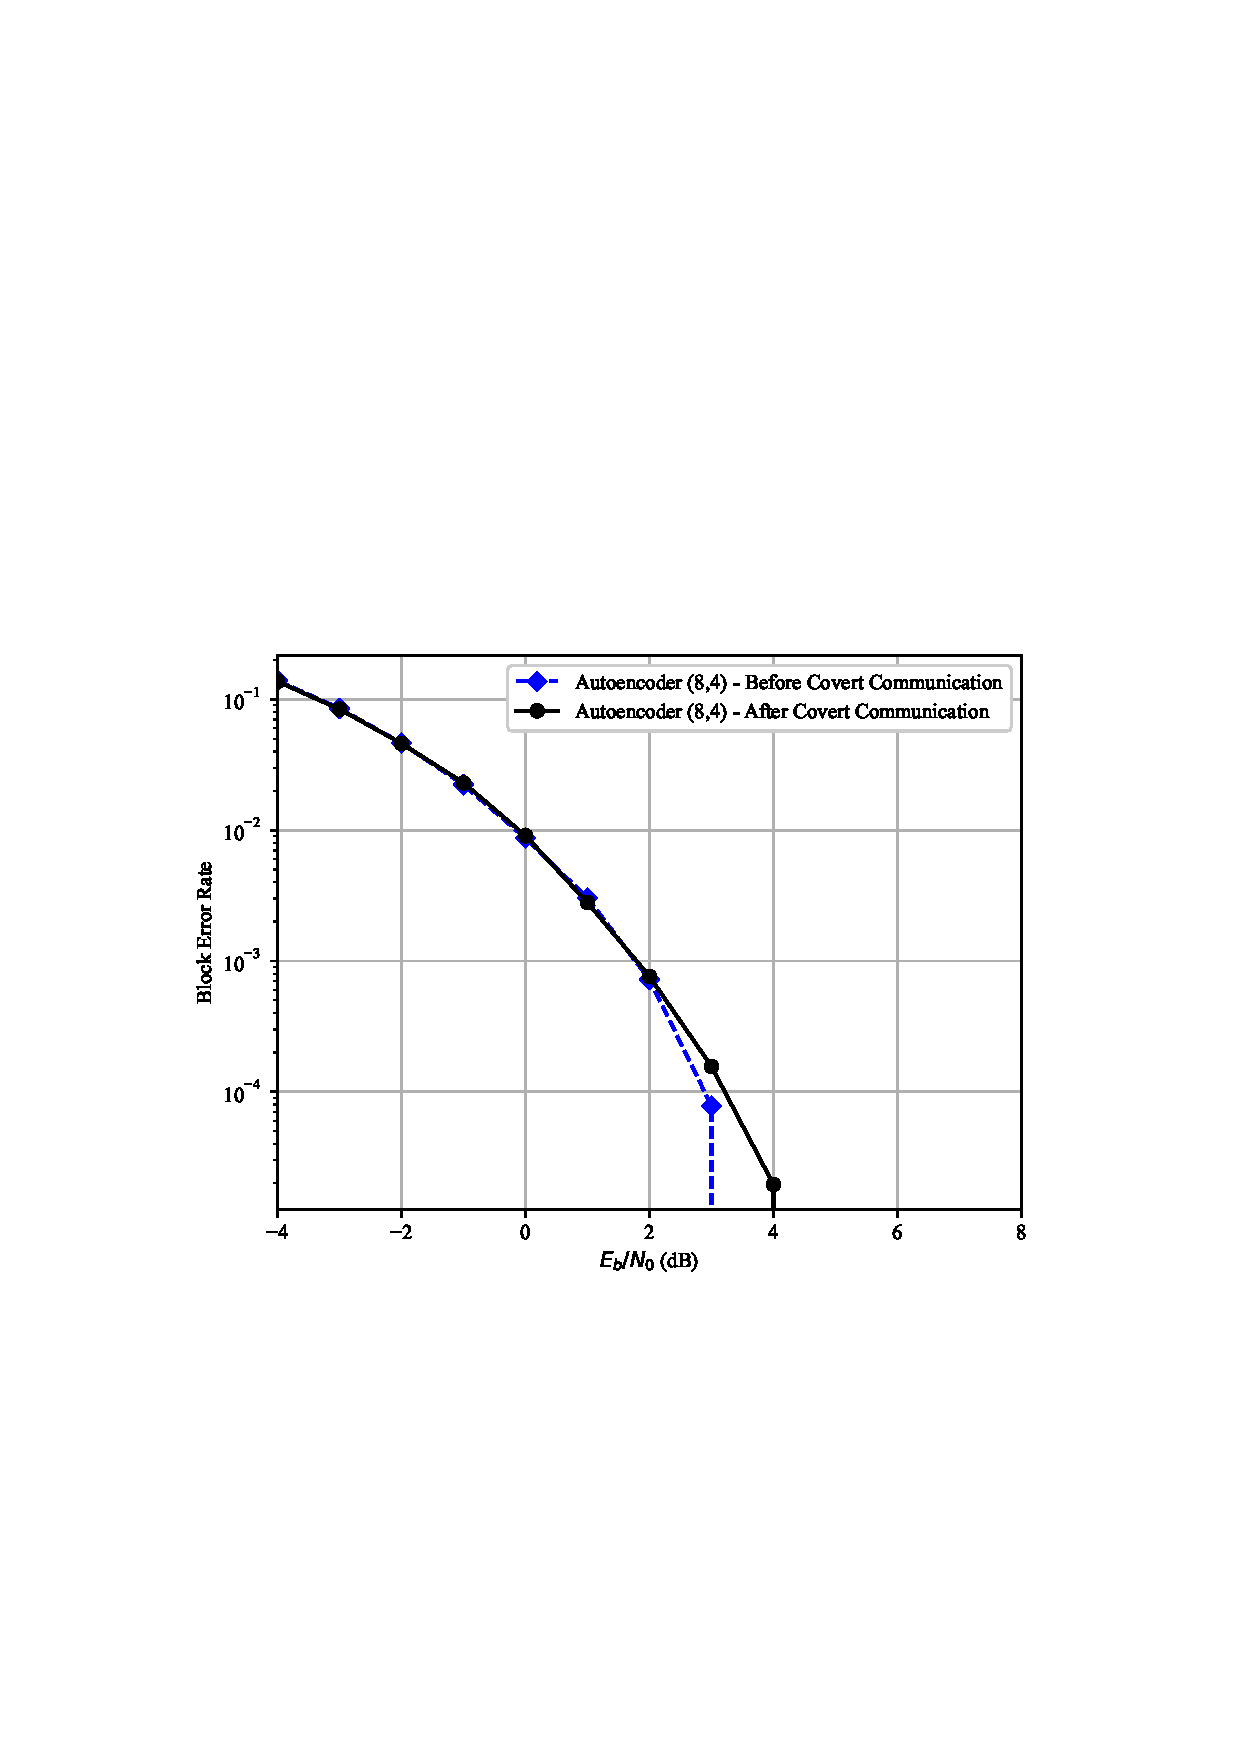
\includegraphics[width=\linewidth]{figs/covert_autoencoder_bler_awgn}
		\caption{Autoencoder's BLER}
		\label{fig:awgn_resutls_ae}
	\end{subfigure}
	\hspace*{\fill}
	\begin{subfigure}{0.3\textwidth}
		\includegraphics[width=\linewidth]{figs/bob_bler_awgn}
		\caption{Bob's BLER}	
		\label{fig:awgn_resutls_bob}
	\end{subfigure}
	\hspace*{\fill}
	\begin{subfigure}{0.3\textwidth}
		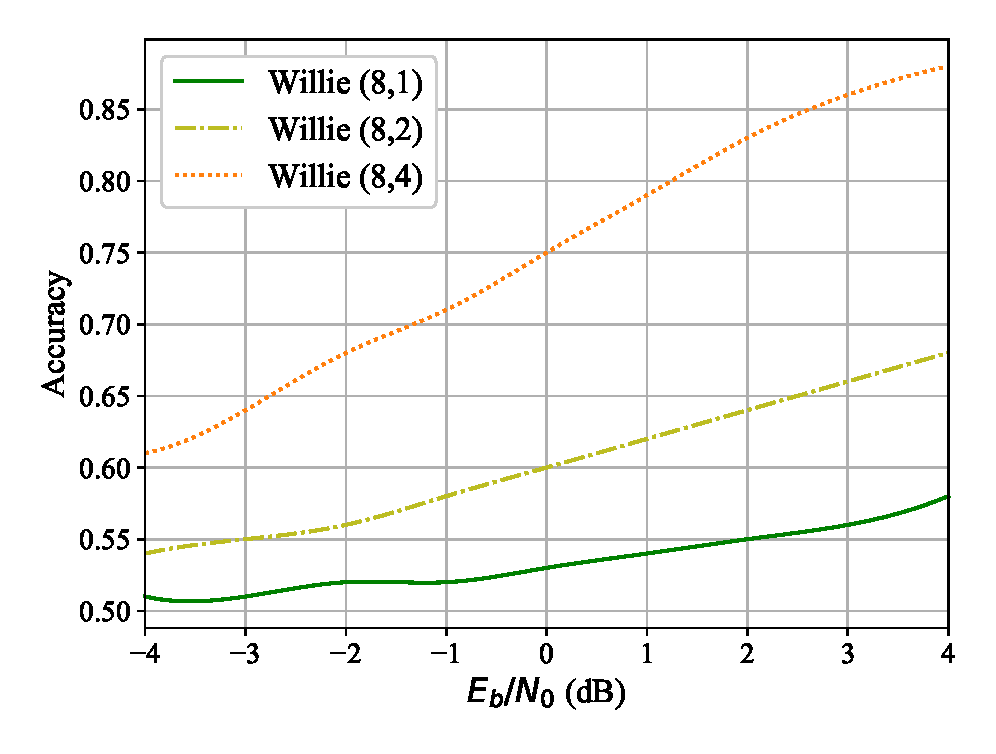
\includegraphics[width=\linewidth]{figs/willie_accuracy_awgn}
		\caption{Willie's accuracy}	
		\label{fig:awgn_resutls_willie}
	\end{subfigure}
	\caption{Trained covert models' performance over AWGN channel for different covert data rates on a range of SNR values.}
	\label{fig:awgn_results}
\end{figure*}
\begin{figure*}
	\begin{subfigure}{0.3\textwidth}
		\includegraphics[width=\linewidth]{figs/covert_autoencoder_bler_rayleigh}
		\caption{Autoencoder's BLER}
		\label{fig:rayleigh_resutls_ae}
	\end{subfigure}
	\hspace*{\fill}
	\begin{subfigure}{0.3\textwidth}
		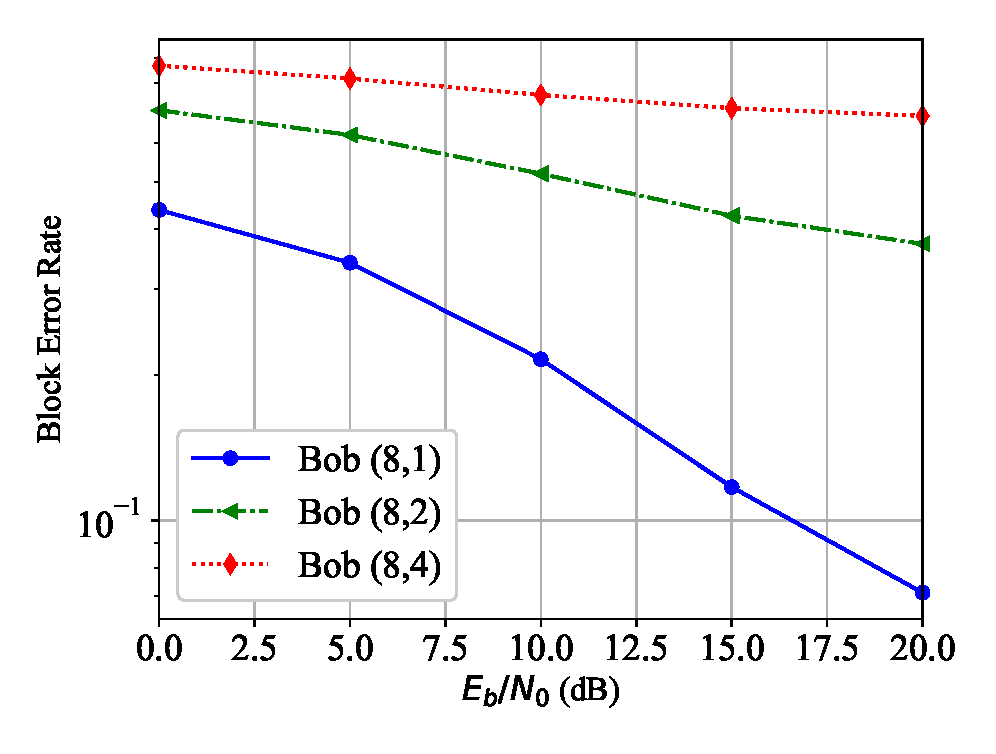
\includegraphics[width=\linewidth]{figs/bob_bler_rayleigh}
		\caption{Bob's BLER}
		\label{fig:rayleigh_resutls_bob}	
	\end{subfigure}
	\hspace*{\fill}
	\begin{subfigure}{0.3\textwidth}
		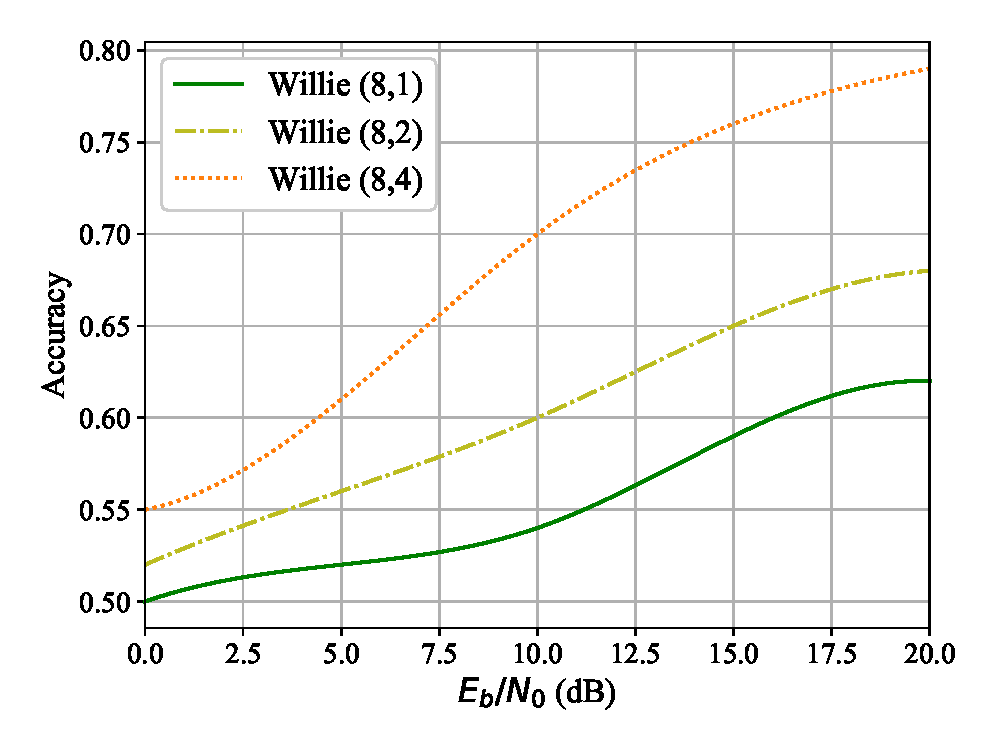
\includegraphics[width=\linewidth]{figs/willie_accuracy_rayleigh}
		\caption{Willie's accuracy}
		\label{fig:rayleigh_resutls_willie}
	\end{subfigure}
	\caption{Trained covert models' performance over Rayleigh fading channel for different covert data rates on a range of SNR values.}
	\label{fig:rayleigh_resutls}
\end{figure*}
\begin{figure*}
	\begin{subfigure}{0.3\textwidth}
		\includegraphics[width=\linewidth]{figs/covert_autoencoder_bler_rician}
		\caption{Autoencoder's BLER}
		\label{fig:rician_resutls_ae}
	\end{subfigure}
	\hspace*{\fill}
	\begin{subfigure}{0.3\textwidth}
		\includegraphics[width=\linewidth]{figs/bob_bler_rician}
		\caption{Bob's BLER}
		\label{fig:rician_resutls_bob}	
	\end{subfigure}
	\hspace*{\fill}
	\begin{subfigure}{0.3\textwidth}
		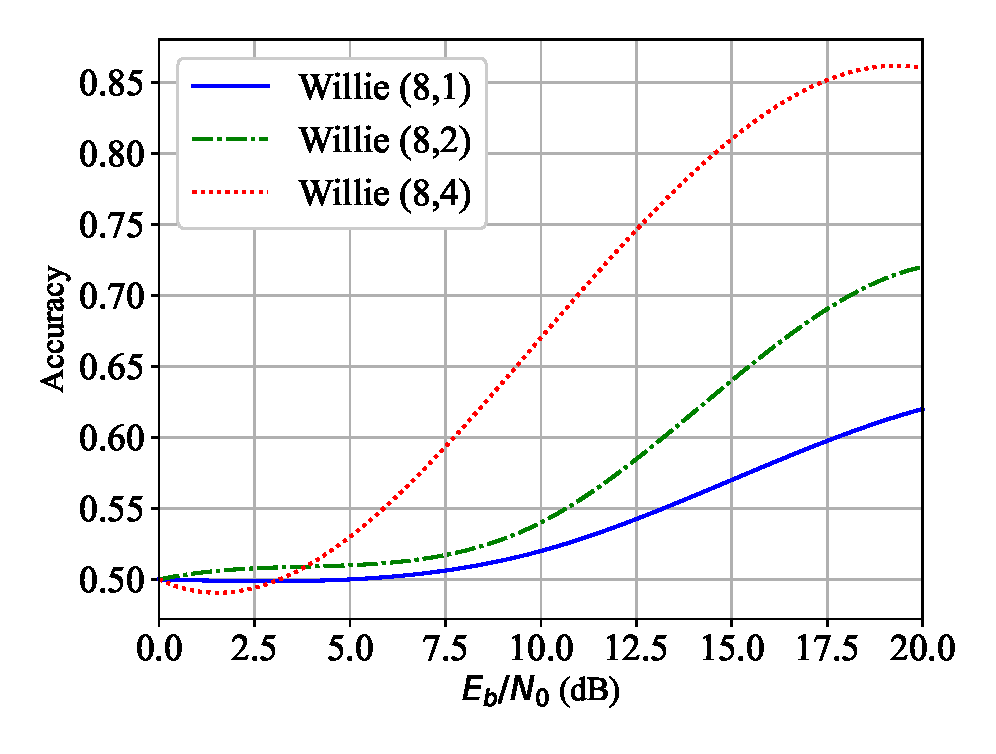
\includegraphics[width=\linewidth]{figs/willie_accuracy_rician}
		\caption{Willie's accuracy}
		\label{fig:rician_resutls_willie}
	\end{subfigure}
	\caption{Trained covert models' performance over Rician fading channel for different covert data rates on a range of SNR values.}
	\label{fig:rician_resutls}
\end{figure*}

\section{Evaluation of Single-User Systems}
\label{s:eval}
We categorize our experiments into two different sections. In the first section, we give performance evaluation information on our trained autoencoder network. Next, we discuss the results of our implemented covert models.


\subsection{Baseline Single-User Autoencoder's Performance}
We implemented an autoencoder communication network for the normal communication between UserRX and UserTX. Based on the notation used in \cite{o2017introduction}, an \(Autoencoder (n, k)\) is a neural network communication model that sends \(k\) bits of data in \(n\) channel uses. We choose these two numbers of channel uses \(n\) and the binary message of size \(k\) to be 8 and 4, respectively. These numbers are chosen this way so that we could evaluate the performance of our trained autoencoder model with the results given in \cite{o2017introduction}. Nevertheless, our covert model works independent of these parameters and can be used for any autoencoder communication setup. In order to train our autoencoder model, we generate two datasets of train and test by generating random binary messages \(s\) of size \(k\). There are 8192 random binary messages in the training set and 51200 random binary messages in the test set. We intentionally created a much larger data set for testing to make sure that each symbol \(y\) undergoes various channel distortions to have an accurate evaluation of the model's performance. We set the learning rate to 0.001 and optimized the model using the Adam optimizer \cite{kingma2014adam}. We choose the batch size to be 64 and train the model for 100 epochs. For the channel configuration, we choose a fixed signal-to-noise ratio (SNR) value during training. The SNR value for the AWGN channel is set to 4dB, 16dB for the Rayleigh and 10db for the Rician fading channels. Figure \ref{fig:autoencoder_bler} shows the performance of our trained normal communication models in terms of block error rate (BLER) for a range of SNR values under AWGN, Rayleigh and Rician fading channel conditions.


\subsection{Covert Model Evaluation Results}
As for the covert models, we evaluate our system's performance on three different channel models of AWGN, Rayleigh fading, and Rician fading. In all settings, we use the same training procedure and network architecture for our covert models. We start our experiment by sending 1 bit of covert data over 8 channel uses and then gradually increase the number of covert bits to see how increasing the covert data rate will affect each component of our covert scheme. The notations \(Alice (n,k)\), \(Bob (n,k)\), and \(Willlie (n,k)\) are used to differentiate models operating on different data rates and the interpretation of it is just the same as what was explained for the autoencoder model. Since each covert message has to be paired with a normal message, we make the train and the test covert messages \(m\) sets to have the same number of train and test messages as the autoencoder's. All models are jointly trained for 5000 epochs using the Adam optimizer. We adjust the importance of each objective for Alice's training by setting \(\lambda_{Willie} = 2 \lambda_{Bob} = 4 \lambda_{UserRX}\) in (\ref{alice_loss}). We start the training with a learning rate of 0.001 and gradually halve the learning rate after every 500 epochs. In each epoch, we first update the parameters of Willie's network using (\ref{willie_loss}), then train Alice's network for one step using (\ref{alice_loss}), and eventually optimize Bob's network based on (\ref{bob_loss}). Although we train our autoencoder network on a fixed SNR value, we find our covert scheme performing better when trained on a range of SNR values. Training our models this way, not only helps Alice to better preserve the normal communication's accuracy but also makes Bob be able to decode covert messages more accurately on lower SNR values. Accordingly, we set the SNR value to be in the range of -2dB to 8dB for the AWGN channel and 10dB to 20dB for both the Rayleigh and the Rician fading channels.

\begin{figure}[tp!]
	\center
	\begin{subfigure}{0.24\textwidth}
		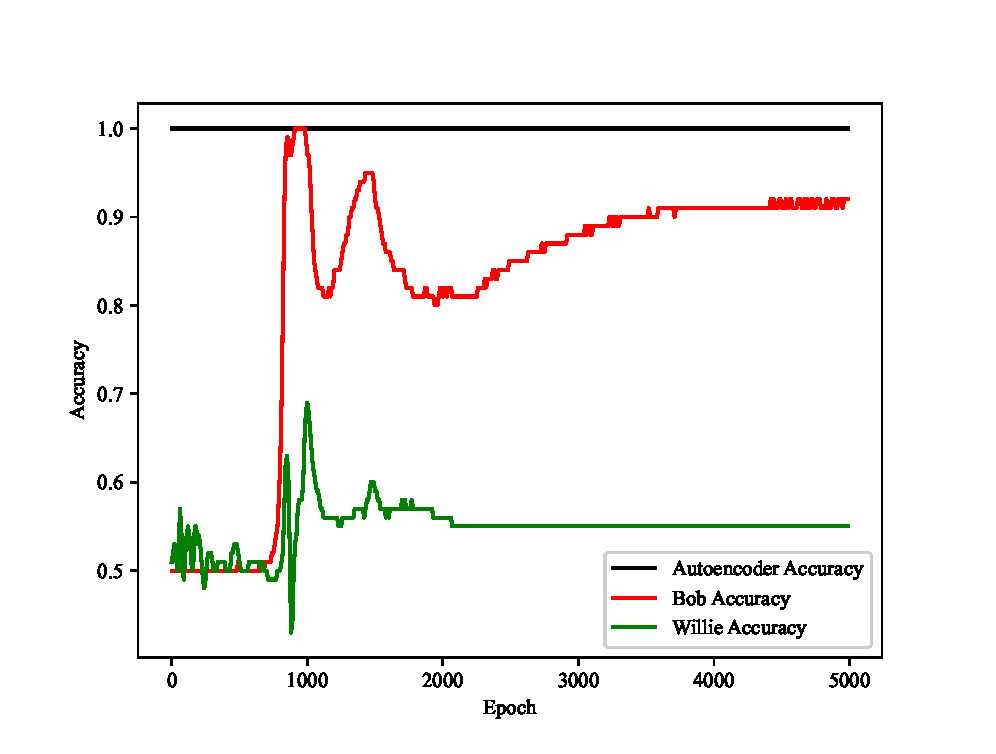
\includegraphics[width=\linewidth]{figs/training_progress_awgn}
		\caption{AWGN channel}
	\end{subfigure}
	\hfill
	\begin{subfigure}{0.24\textwidth}
		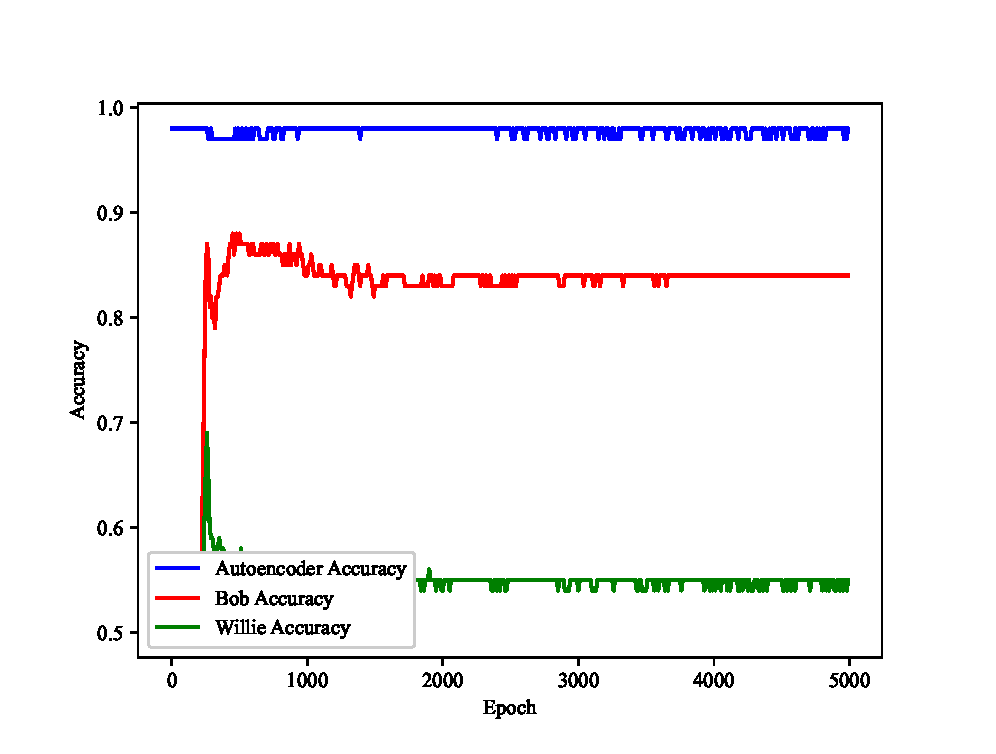
\includegraphics[width=\linewidth]{figs/training_progress_rayleigh}
		\caption{Rayleigh fading channel}	
	\end{subfigure}
	\begin{subfigure}{0.24\textwidth}
	\includegraphics[width=\linewidth]{figs/training_progress_rician}
	\caption{Rician fading channel}	
	\end{subfigure}
	\caption{Evaluation results of our covert and autoencoder models during the training process show the system reaches a stable point after successful training.}
	\label{fig:traning_progress}
\end{figure}


\textbf{Training Procedure}: Figure \ref{fig:traning_progress} shows the progress of each covert actor's accuracy on the test set during the training process. As the training goes on, Bob gradually learns to decode covert messages \(m\) and establishes a reliable communication with Alice. After a few epochs, when the covert communication starts to take form and stabilizes, signals start to deviate from the distribution they had, causing Willie to better detect covert signals. When Willie's accuracy increases, the term \(\mathcal{L}_{Willie}\) dominates the other two objectives of Alice's loss function in (\ref{alice_loss}). This causes Alice to gradually sacrifice its accuracy for the sake of undetectability. Soon afterwards, the training process reaches a stable point where neither of the covert models sees any noticeable improvement in their accuracy as the training continues. 


\textbf{Covert Rate}: Figures \ref{fig:awgn_results}, \ref{fig:rayleigh_resutls}, and \ref{fig:rician_resutls} show our final results. It also demonstrates how the accuracy of each of our covert models changes as we increase the covert rate. As we expected, covert communication becomes more unreliable, impact on normal communication increases, and detection becomes easier at higher covert rates.


\textbf{Undetectibility}: In figures \ref{fig:awgn_resutls_willie}, \ref{fig:rayleigh_resutls_willie}, and \ref{fig:rician_resutls_willie} the accuracy of Willie is shown in percentage over a range of SNR values for flagging signals as covert and normal. These plots give us some intuition on how probable it will be for our covert signals to be detected by a target detector at each SNR value for different covert rates. Figures \ref{fig:awgn_constellation},\ref{fig:rayleigh_constellation}), and \ref{fig:rician_constellation} compare the constellation cloud of a covert and a normal signal for AWGN, Rayleigh and Rician fading channels. We have marked each symbol of the encoder's output signal \(x\) as black circle points on the constellation diagrams. The red constellation cloud shows how covert signals scatter after going through the channel and the green cloud shows this for normal signals. Since data is sent over 8 channel uses, there are 8 black points on the chart. To be consistent with Willie's accuracy and Bob's error rate for our both channel models, we have set the SNR value to 2dB for the AWGN and 15dB for the Rayleigh fading channel and 8db for the Rician fading channel so that in all channel models, the probability of detection remains relatively the same and the covert communication BLER stays below \(10^{-1}\). This area of operation gives Alice and Bob fair covert communication reliability while maintaining their covertness. As it is also evident in these figures, comparing the signal constellation diagrams before and after our covert model applied shows that Alice has perfectly learned to cloak the covert signals into the distribution of the channel's noise after a successful training procedure.

\begin{figure}[bp!]
	\begin{subfigure}{0.24\textwidth}
		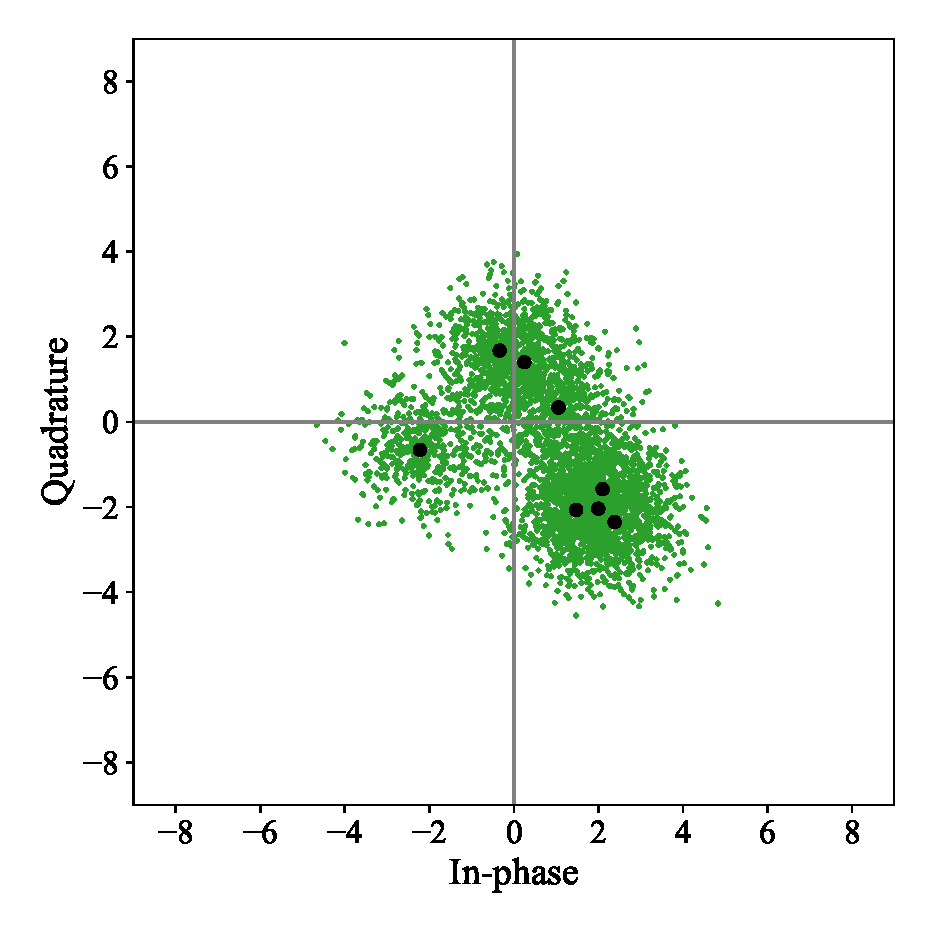
\includegraphics[width=\linewidth]{figs/awgn_normal_constellation}
		\caption{Without covert transmission}
	\end{subfigure}
	\hfill
	\begin{subfigure}{0.24\textwidth}
		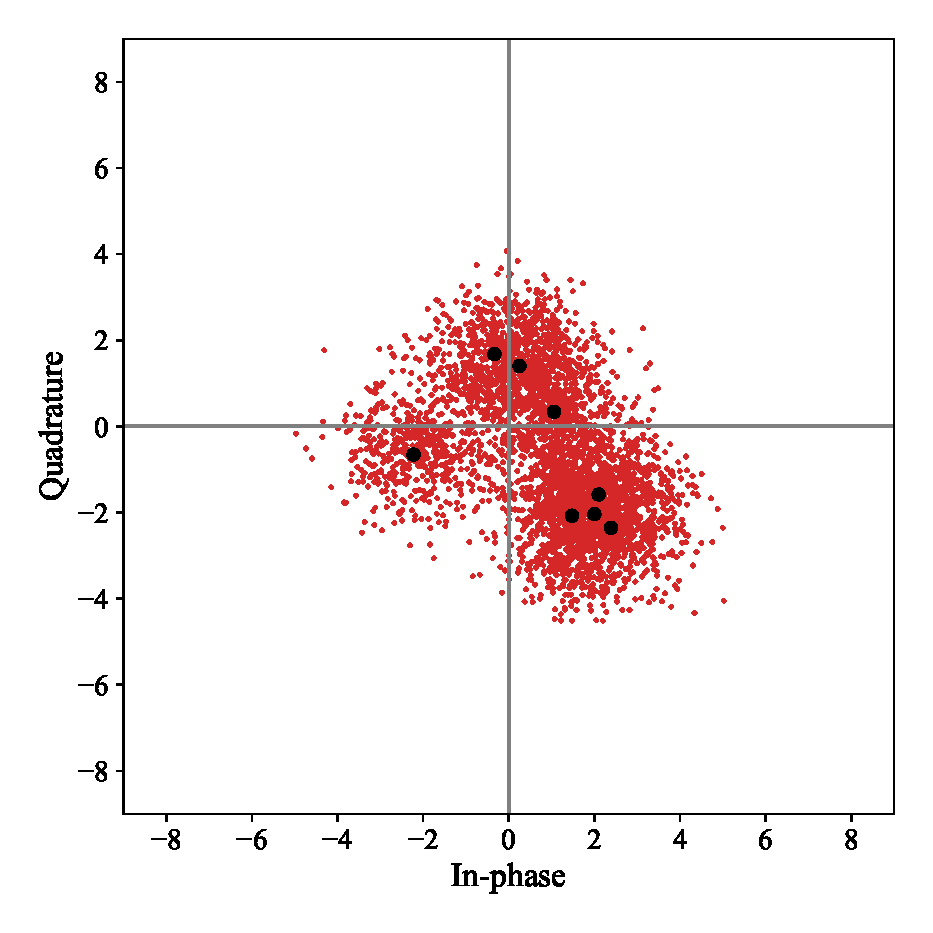
\includegraphics[width=\linewidth]{figs/awgn_covert_constellation}
		\caption{With covert transmission}	
	\end{subfigure}
	\caption{Comparing AWGN channel constellation clouds of a signal before and after our covert scheme is applied.}
	\label{fig:awgn_constellation}
\end{figure}
\begin{figure}[bp!]
	\begin{subfigure}{0.24\textwidth}
		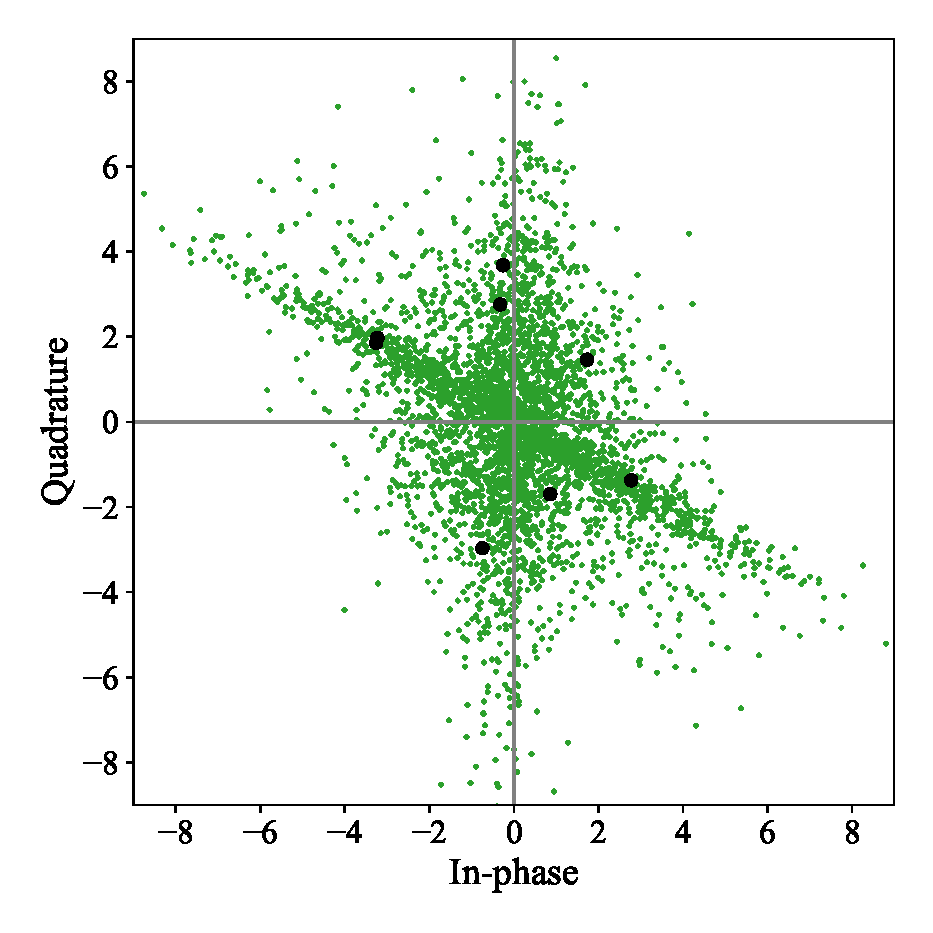
\includegraphics[width=\linewidth]{figs/rayleigh_normal_constellation}
		\caption{Without covert transmission}
	\end{subfigure}
	\hfill
	\begin{subfigure}{0.24\textwidth}
		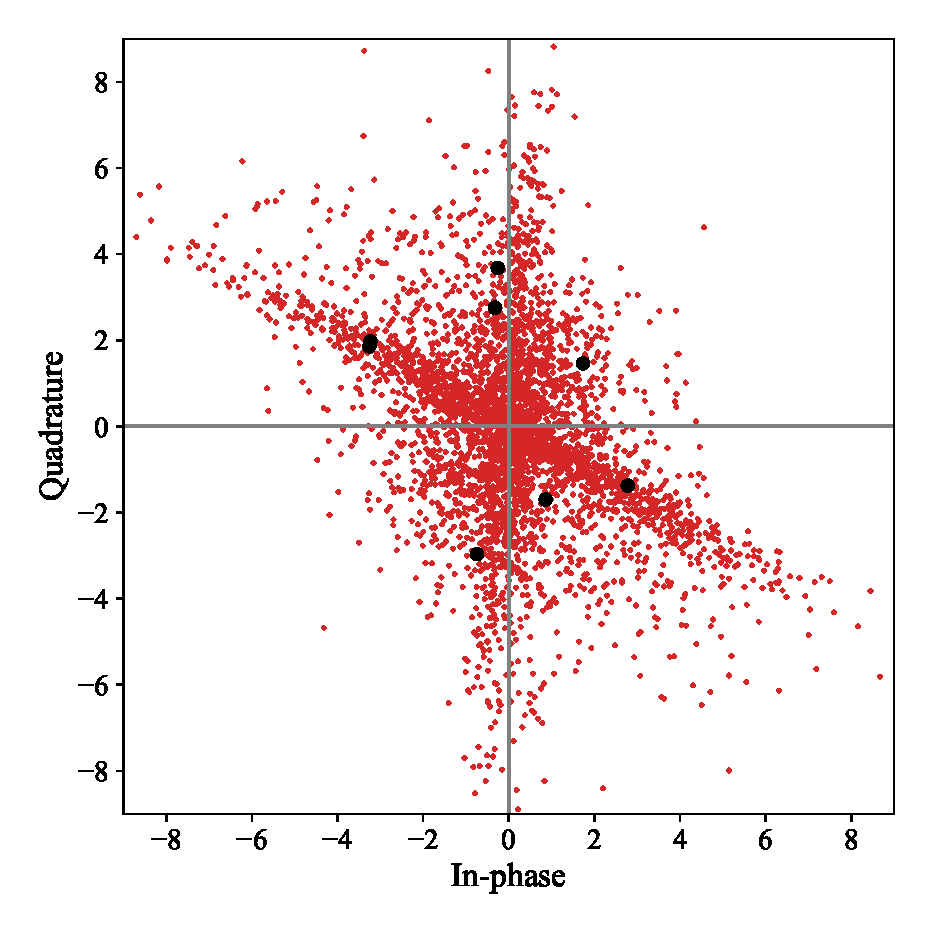
\includegraphics[width=\linewidth]{figs/rayleigh_covert_constellation}
		\caption{With covert transmission}	
	\end{subfigure}
	\caption{Comparing Rayleigh fading channel constellation clouds of a signal before and after our covert scheme being applied.}
	\label{fig:rayleigh_constellation}
\end{figure}
\begin{figure}[bp!]
	\begin{subfigure}{0.24\textwidth}
		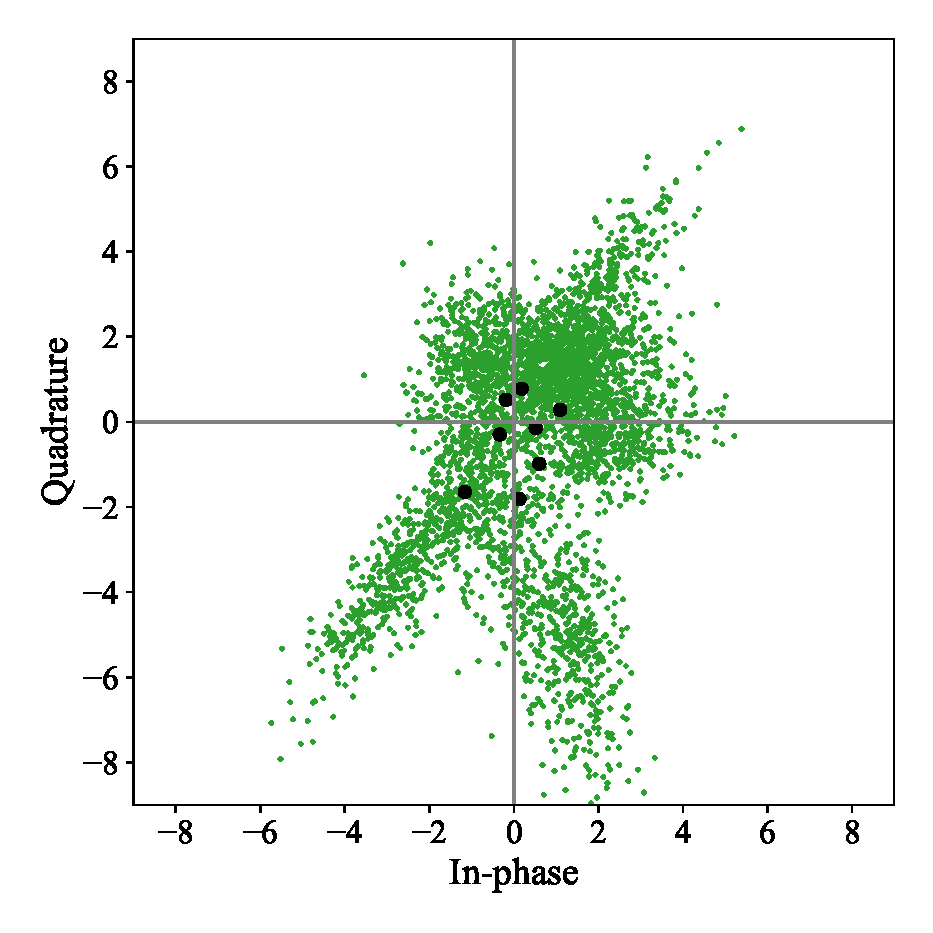
\includegraphics[width=\linewidth]{figs/rician_normal_constellation}
		\caption{Without covert transmission}
	\end{subfigure}
	\hfill
	\begin{subfigure}{0.24\textwidth}
		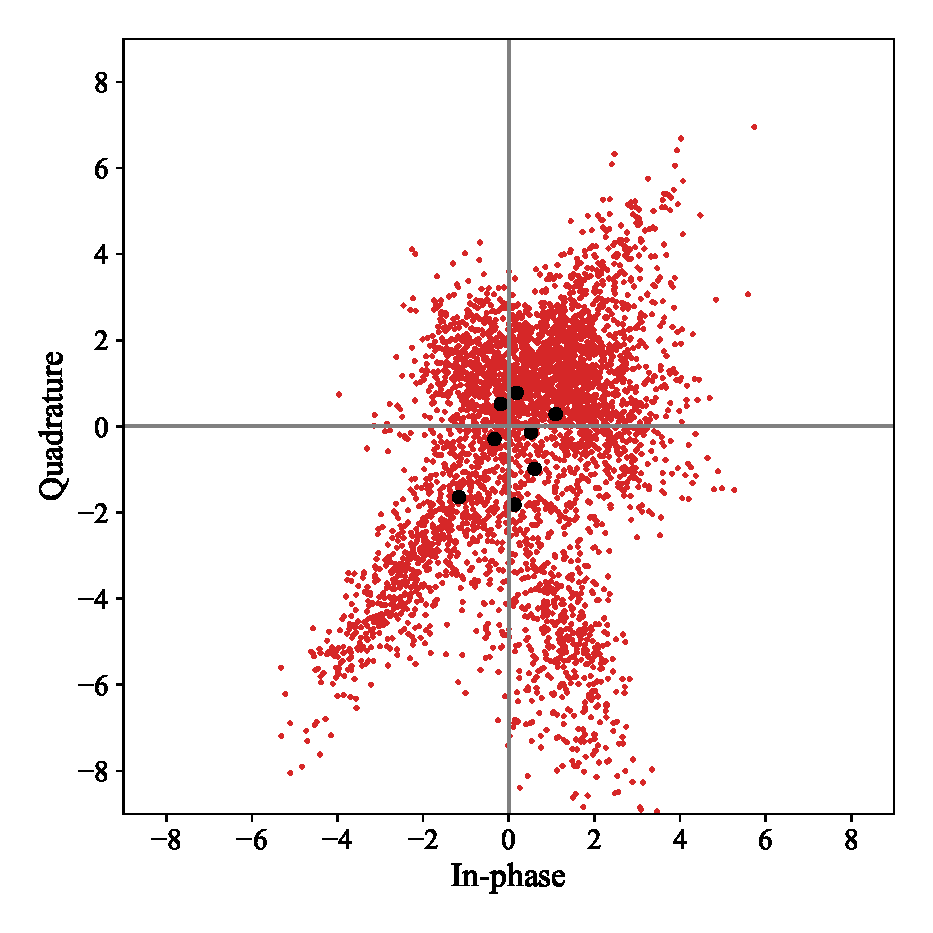
\includegraphics[width=\linewidth]{figs/rician_covert_constellation}
		\caption{With covert transmission}	
	\end{subfigure}
	\caption{Comparing Rician fading channel constellation clouds of a signal before and after our covert scheme being applied.}
	\label{fig:rician_constellation}
\end{figure}
\begin{figure*}[thp]
	\center
	\begin{subfigure}{0.75\textwidth}
		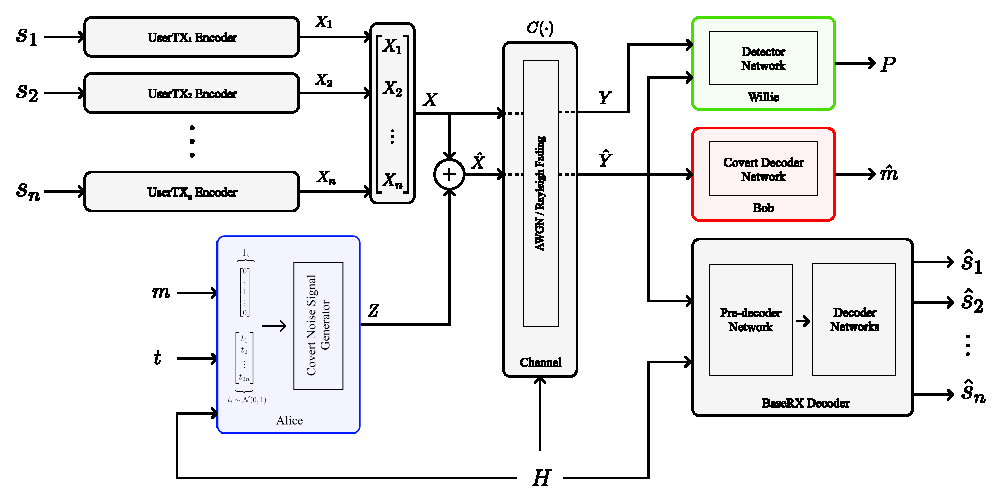
\includegraphics[width=\linewidth]{figs/multi_system_architecture}
	\end{subfigure}
	\\
	\caption{Overall architecture of our system model in the multi-user scenario. Alice is communicating with Bob by generating covert noise signals without disturbing the communication between other \(n\)-UserTXs and BaseRX; meanwhile, Willie tries to distinguish covert and normal signals (Colored components are under the control of covert users and gray components are the non-modifiable parts of the system).}	
	\label{fig:multi_system_architecture}
\end{figure*}


\section{Multi-User System Model}
\label{s:multi-model}
Now that we discussed the single-user system model and evaluation results, in this section, we are going to talk about the second part of our article that covers a multi-user communication model scenario. Many parts of this model will be similar to what we described in (=\ref{s:single-model}) except that with more than one user sharing the channel, both normal and covert users now have to account for signal interference to communicate reliably. This will result in a much more complex optimization problem when we are training normal and covert users' neural networks.

In figure \ref{fig:multi_system_architecture} you can see the overall architecture of our multi-user communication system. The system compromises multiple separate normal transmitters (UserTXs) that are sending signals to a central base station receiver (BaseRX). Each UserTX and BaseRX together form an autoencoder model wherein UserTX is the encoder and BaseRX acts as the decoder network. The objective of our work, again, is to establish a covert channel between two covert users, namely Alice and Bob, on top of this normal communication channel without leaving any impact on any of these normal communicating parties. Normal transmitters each use their own encoder network to encode a binary message to a vector of signals. Their networks share no parameters and the message they are sending is unknown to the other transmitters of the system. At the time of transmission, they all send their signals simultaneously and since they are sharing the same channel, there will be channel interference. As for the channel effect, the two channel models of AWGN and Rayleigh fading are considered. When signals pass through the channel, they get distorted both by the channel effects and the channel interference. These noisy signals are then received at BaseRX, all at the same time. BaseRX uses its decoder network to reconstruct the messages sent by the transmitters from the received signals. Alice and Bob's objective is no different from what we mentioned previously in our single-user system model. Their goal is to construct a hidden communication channel and embody their messages inside normal signal transmissions of the communication system in form of an added noise. In order to remain covert, they have to ensure that these added perturbations make no disturbance to the ongoing normal communication (i.e. increasing the error rate of communication) and leave no statistical traces behind from an observer's perspective. Thus, there is an observer (Willie) whose objective is to continuously look into the transmitted signals over the channel and raise an alarm whenever covert communication is deemed to be present. We represent all these roles by DNNs that are collaboratively trained to establish a covert communication channel. By using a generative model, Alice embeds its confidential message into a covert noise vector which will be added to the signals being transmitted over the channel. Bob receives this signal and uses its decoder network to extract the covert message. Unlike our single-user system model wherein covert users were devised independently of what the channel model is, here they use different neural networks depending on the channel model. Channel statistics are monitored by the observer of the system (Willie). Willie's objective is to detect any anomaly that in this case would be a covert communication taking place. Thus, if Alice and Bob construct their covert signals in such a way that Willie fails to tell them apart from the normal signals, then the covertness of their communication is safeguarded.

\textbf{Background on Multi-User Autoencoder Systems}: A multi-user autoencoder communication system is just an extended version of a single-user system with either multiple transmitters and receivers or multiple transmitters and a central receiver. We considered the latter in our work. Similar to the single-user system, in this model each of these encoders (transmitters) first maps \(k\) bits of data into a message \(s_i\) where \(s \in \{1,...,M\}\), \(M = 2^k\), and \(i\) is the index of the transmitter. Then each transmitter takes this transformed message as an input and generates a signal \(x_i = E_i(s_i) \in \mathbb{R}^{2n}\), which is a real-valued vector. This \(2 \times n\)-dimensional real-valued vector can be treated as an \(n\)-dimensional complex vector where \(n\) is the number of channel uses that are needed for the signal to be transmitted over. Next, there will be distortions caused by the channel interference and effects. For the AWGN channel, transmitted signals are added together and the channel's noise effect \(z\) gets added to this mixed signal vector. Thus, each transmitter's received signal at the receiver, carrying the noise of the channel and interference, can be expressed as \(y_i = \sum_{i=0}^{m}x_i + z_i\) where \(n_{tx}\) is the number of transmitters. In Rayleigh fading channel case, signals are simultaneously faded and mixed by being multiplied by the channel matrix and the resulting vector of signals for each transmitter can be expressed as \(y_i = h_i \cdot x + z_i\), where \(h_i\) is channel coefficients for the \(i^{th}\) transmitter's signals (\(h\) itself is a vector of size \(n_{tx}\) wherein each element \(h_{i_j}\sim \mathcal{CN}(0, 1)\)) and \(x\) is a vector containing all transmitters' encoded signals. Transmitted signals that have gone through the channel are received at the decoder (receiver) and then get passed to a transformation function \(D: \mathbb{R}^{2n} \rightarrow M \) along with the channel matrix \(h\) and eventually, the reconstructed version of the message \(s\), which is denoted as \(\hat{s} = D(y, h)\), is obtained.

\begin{figure*}[!tp]
	\center
	\begin{subfigure}{0.45\textwidth}
		\includegraphics[width=\linewidth]{figs/multi_autoencoder_bler_awgn}
		\caption{AWGN channel}
	\end{subfigure}
	\begin{subfigure}{0.45\textwidth}
		\includegraphics[width=\linewidth]{figs/multi_autoencoder_bler_rayleigh}
		\caption{Rayleigh fading channel}	
	\end{subfigure}
	\caption{Trained Autoencoders' BLERs for different numbers of users over a range of SNR values in our multi-user system.}
	\label{fig:multi_autoencoder_bler}
\end{figure*}


\section{Covert Model for Multi-User Systems}
The covert communication starts with Alice sending a binary secret message \(m\) to Bob. This message is first encoded to a one-hot vector and then passed to a generator network to produce a covert signal noise signal \(\hat{z}\). This then will be added to a vector of normal signals \(x\), which contains signals from all the transmitters before transmission. Hence, the resulting covert signal can be denoted as:
\begin{equation}
	\hat{x}_i = x_i + \hat{z}.
\end{equation}

Afterwards, this signal is transmitted over the channel. We have considered two channel models of AWGN and Rayleigh for this model. Each of these channel models has an effect on the signal that we denote as a mapping function \(C(\cdot)\).

\textit{AWGN Channel Output}: In this channel mode, the channel effect is applied by adding a noise vector \(z \sim \mathcal{N}(0, \sigma_{chl}^2)\) to the signal. Therefore, the channel function \(C(\cdot)\) and the channel output \(\hat{y}\) can be represented as:
\begin{equation}
	\hat{y}_i = C(\hat{x}_i) = \sum_{i=0}^{m}\hat{x}_i + z_i.
\end{equation}

\textit{Rayleigh Channel Output}: For the Rayleigh fading channel model, a flat block fading channel is considered wherein each code-word \(\hat{x}_i\) is assumed to be faded independently by fading coefficient \(h_{i_j}\). Consequently, the channel function \(C(\cdot)\) and the final covert signal \(\hat{y}\) is written as:
\begin{equation}
	\hat{y}_i = C(\hat{x}_i) = h_i \cdot \hat{x} + z_i.
\end{equation}

After the signal goes through the channel, Bob receives it at its receiver. With the help of his decoder network, he extracts the covert message \(\hat{m}\) from the covert signal \(\hat{y}\). Similarly, BaseRX receives the same signal and passes it to its decoder to reconstruct the message \(\hat{s}\).

Willie as an observer of the system continuously monitors the channel. His job is to label the received signals as covert and normal. By gradually altering the covert signals and tracking how Willie's confidence in detecting covert signals changes, Alice will steadily learn to better cover up its covert signals. Technically, Alice tries to make covert signals statistically similar to normal signals so that they become indistinguishable.

\subsection{General Formulation}

To have reliable working covert communication between Alice and Bob, Bob needs to learn how to decode the messages that Alice transmits. In this regard, the first objective of Bob is to minimize the reconstruction error of the covert message \(m\) sent by Alice. Similar to what we proposed in our single-model system, Alice maps binary covert messages \(m\) to a vector of covert signals \(\hat{z}\) using a generative model. The only difference in Alice's network from before is that now Alice needs the channel matrix \(h\) when she is operating over Rayleigh fading channel. Therefore, given \(A(\cdot)\) as Alice's generative model, the produced covert signal for AWGN and Rayleigh channels are \(\hat{z}_{m, t} = A(m, t)\), \(\hat{z}_{m, t, h} = A(m, t, h)\), respectively. Now let \(B(\cdot)\) be the function of Bob's decoder network, then below loss function ensures the above objective:
\begin{equation}
	\begin{aligned} \label{multi_bob_loss}
		\mathcal{L}_{Bob} & = \mathbb{E}_{m}[H(\hat{m}, m)] \\
		& = \mathbb{E}_{m}[H(B(\hat{y}), m)] \\ 
		& = \mathbb{E}_{m}[H(B(C(\hat{x}), m)] \\ 
		& = \begin{cases} 
			\mathbb{E}_{m}[H(B(C(A(m, t) + x)), m)] & AWGN \\
			\mathbb{E}_{m}[H(B(C(A(m, t, h) + x)), m)] & Rayleigh.
			\end{cases}
	\end{aligned}
\end{equation}

We use this equation to train both Alice's and Bob's networks by freezing one or the other's network parameters. From an observer's point of view, any abnormal increase in communication's error rate would indicate an anomaly in the system and in our case a covert communication. Therefore, Alice needs to tune its covert signals so that its impact on other normal transmitters communication is minimum. This we will achieve by using the below loss function for Alice's network:
\begin{equation}
	\begin{aligned} \label{multi_alice_user_loss}
		\mathcal{L}_{BaseRX} & = \sum_{i=0}^{i=m}\mathbb{E}_{m}[H(\hat{s}_i, s_i)] \\
		& = \sum_{i=0}^{i=m}\mathbb{E}_{m}[H(D(\hat{y}_i), s_i)] \\
		& = \sum_{i=0}^{i=m}\mathbb{E}_{m}[H(D(C(\hat{z}_i + x_i)), s_i)] \\
		= \sum_{i=0}^{i=m} & \begin{cases} 
			\mathbb{E}_{m}[H(D(C(A(m, t) +  x_i)), s_i)] & AWGN \\
			\mathbb{E}_{m}[H(D(C(A(m, t, h) + x_i), h), s_i)] & Rayleigh. \\
		\end{cases} 
	\end{aligned}
\end{equation}
 
With the two equations above, the reliability of covert communication will be achieved and we will have covertness to some extent. Yet, we need to account for an observer (Willie) who will be appointed to observe the communication channel closely to detect if any probable covert or abnormal communication is taking place. Thus, there is a third loss function for Willie denoted as:
\begin{equation}
	\begin{aligned} \label{multi_willie_loss}
		\mathcal{L}_{Willie} & = \mathbb{E}_{m}[H(\hat{y}, y)] \\
		& = \mathbb{E}_{m}[H(C(\hat{x}), C(x))] \\
		& = \begin{cases}
			\mathbb{E}_{m}[H(C(A(m,t) + x), C(x))] & AWGN \\
			\mathbb{E}_{m}[H(C(A(m,t,h) + x), C(x))] & Rayleigh.
			\end{cases}
	\end{aligned}
\end{equation}

Using this loss function, Willie will have enough data to learn how to differentiate covert and normal signals. Since it is vital for covert users to keep their transmissions hidden from the observer of the system, they can exploit the same loss function declared above to increase the covertness of their communication. By putting these constraints all together and using equation (\ref{alice_loss}), we now have the final optimization formula for training Alice's network.

\subsection{Neural Network Architecture}
There is not much difference in our models' architectures from what we proposed in the single-user model except for the decoder part of the autoencoder's network and a few extra parameters for Alice's network. We will explain each model's structure in detail in the following subsections.

\textbf{Autoencoders' Networks}: The input to each autoencoder model is a different binary message \(s\) of size \(k\) bits and the output is a reconstructed version of that message \(\hat{s}\). Figure \ref{fig:mutli_autoencoder_architecture} depicts the overall architecture of our multi-user autoencoder model. First, each autoencoder model transforms the given message into its one-hot representation and then encodes it to a vector of signals of size \(2 \times n\), where \(n\) is the number of channel uses for the whole system. Signals are then distorted using a mapping function that corresponds to the channel model effects. On the receiver side, there is a central decoder that receives all transmitter's signals at once and extracts the message of each by passing the signals through its neural network. When the channel model is Rayleigh fading, the decoder equalizes the signals using zero-forcing technique with the channel matrix before passing the signals to its network. Note that there are plenty of more complex equalization functions that can be used, however, optimizing the performance of the autoencoder model is not the focus of this article.

\textbf{Alice's Network}: Alice takes a random trigger \(t\), and a covert message \(m\), which is one-hot encoded, and then uses her generator model to produce a covert noise signal \(\hat{z}\). In the case of the Rayleigh fading channel, the channel matrix is also fed to her network. Next, she adds this to normal signals \(x_i\)s that are carrying the normal messages between normal users of the system. Alice's generator model consists of dense layers with ReLU and Tanh activation functions. The first layer of her model takes a trigger input \(t\), a covert message \(m\). Channel matrix \(h\) is also an input to her network when the channel is Rayleigh fading. Followed are multiple fully connected layers that are to extract the useful features and do the encoding process. The last layer of the network does a dimension transformation so that the generated covert signal \(\hat{z}\) complies with the dimension of normal signals \(x_i\)s on the channel. 

\textbf{Bob's Network}: A noisy version of covert signal \(\hat{y}\) is received at Bob's decoder network. His objective is to extract the secret message by doing classification on the signal. This received signal first goes through the first layer of his network, which is a wide dense layer with a Tanh activation function, and its aim is to increase the input's feature space. Then the data is passed through multiple 1-Dimensional Convolutional (1D Conv) layers that allow Alice and Bob to develop a mutually learned coding. The last two dense layers of Bob's network are for domain remapping from the learned feature space to the covert message domain space. After a successful training, Bob will eventually learn to decode the messages from covert signals by doing classification.


\textbf{Willie's Network}: Whatever signal Bob receives, Willie receives as well. He also has access to the normal signals \(y\) and by doing binary classification on these signals and the covert signals \(\hat{y}\), he outputs a probability vector \(P\) that shows how probable it is for the signals to be normal or covert. Willie's network architecture is chosen to be the same as the Bob's except for the last layer, which has a Sigmoid activation function instead of a Softmax. By having equally sized networks, we can ensure that Bob and Willie will have the same capacity for learning, and thus can compete in a fair way.

\begin{figure}[tp!]
	\center
	\begin{subfigure}{0.5\textwidth}
		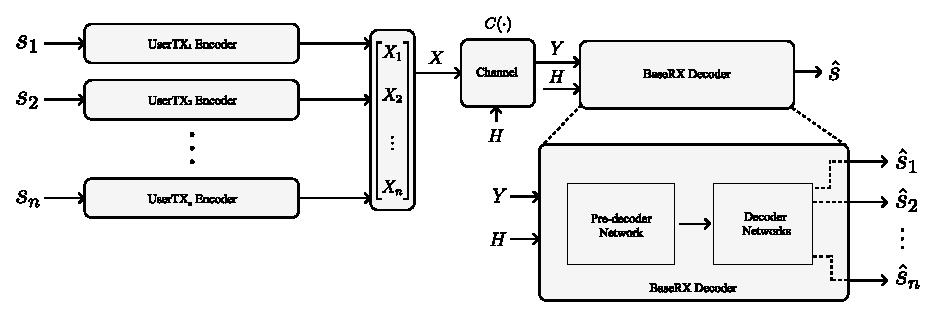
\includegraphics[width=.98\linewidth]{figs/multi_autoencoder_architecture}
	\end{subfigure}
	\\
	\caption{Detailed architecture of BaseRX's decoder network. Signals from all receivers are passed through the pre-decoder network and then each transmitter's message is extracted separately using the decoder networks.}	
	\label{fig:multi_autoencoder_architecture}
\end{figure}
\begin{figure*}[tp!]
	\begin{subfigure}{0.3\textwidth}
		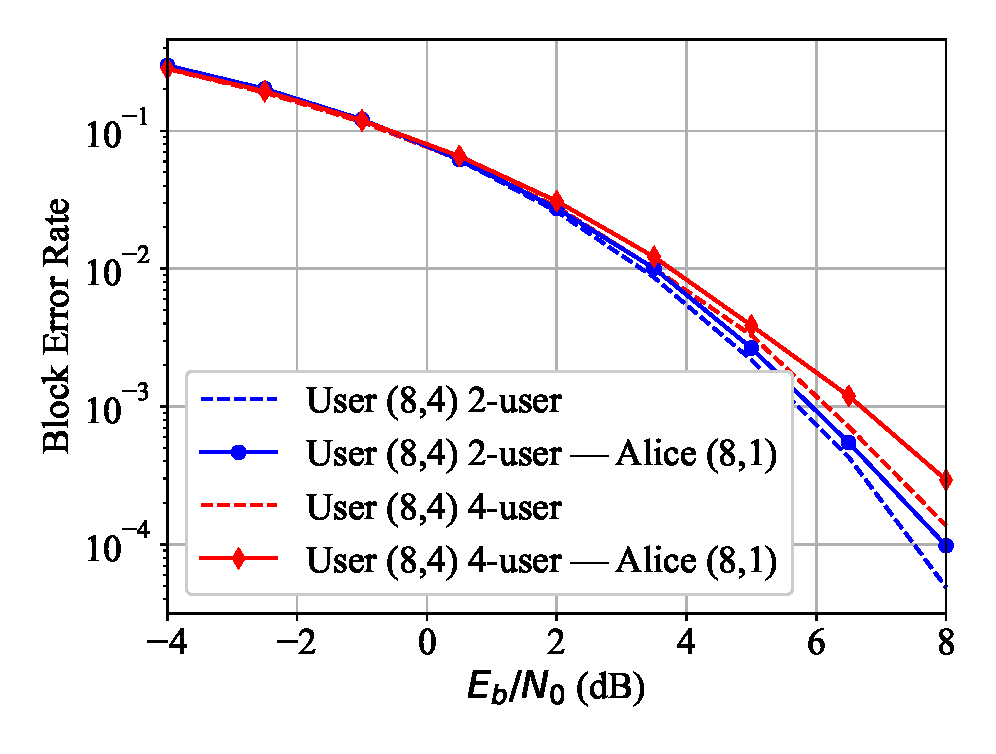
\includegraphics[width=\linewidth]{figs/multi_covert_autoencoder_bler_awgn}
		\caption{Autoencoder's BLER}
		\label{fig:multi_awgn_resutls_ae}
	\end{subfigure}
	\hspace*{\fill}
	\begin{subfigure}{0.3\textwidth}
		\includegraphics[width=\linewidth]{figs/multi_bob_bler_awgn}
		\caption{Bob's BLER}	
		\label{fig:multi_awgn_resutls_bob}
	\end{subfigure}
	\hspace*{\fill}
	\begin{subfigure}{0.3\textwidth}
		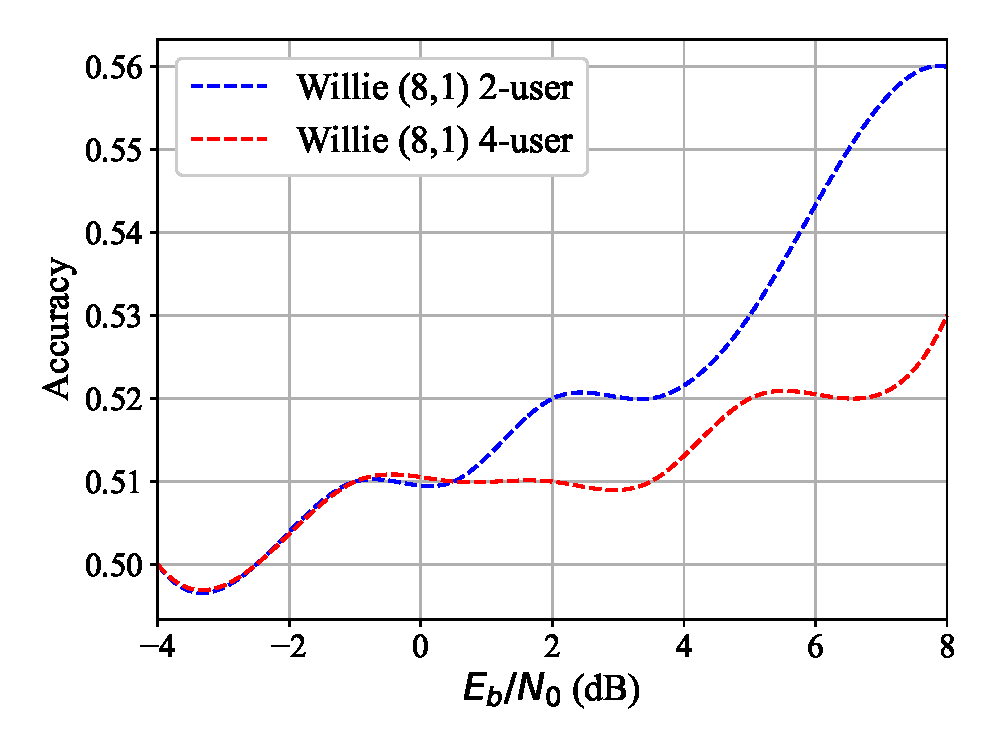
\includegraphics[width=\linewidth]{figs/multi_willie_accuracy_awgn}
		\caption{Willie's accuracy}	
		\label{fig:multi_awgn_resutls_willie}
	\end{subfigure}
	\caption{Trained covert models' performances over AWGN channel for systems with different numbers of users on a range of SNR values.}
	\label{fig:multi_awgn_results}
\end{figure*}
\begin{figure*}
	\begin{subfigure}{0.3\textwidth}
		\includegraphics[width=\linewidth]{figs/multi_covert_autoencoder_bler_rayleigh}
		\caption{Autoencoder's BLER}
		\label{fig:multi_rayleigh_resutls_ae}
	\end{subfigure}
	\hspace*{\fill}
	\begin{subfigure}{0.3\textwidth}
		\includegraphics[width=\linewidth]{figs/multi_bob_bler_rayleigh}
		\caption{Bob's BLER}
		\label{fig:multi_rayleigh_resutls_bob}	
	\end{subfigure}
	\hspace*{\fill}
	\begin{subfigure}{0.3\textwidth}
		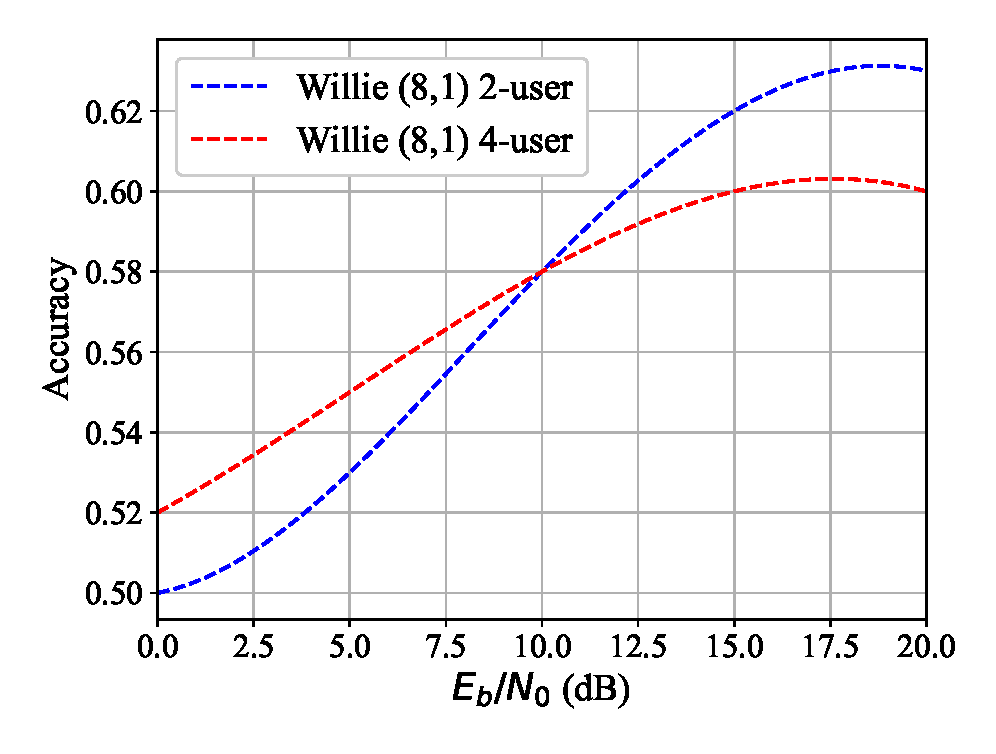
\includegraphics[width=\linewidth]{figs/multi_willie_accuracy_rayleigh}
		\caption{Willie's accuracy}
		\label{fig:multi_rayleigh_resutls_willie}
	\end{subfigure}
	\caption{Trained covert models' performances over Rayleigh fading channel for systems with different number of users on a range of SNR values.}
	\label{fig:multi_rayleigh_resutls}
\end{figure*}

\begin{table}[bp!]
	\begin{adjustbox}{width=0.9\columnwidth,center}
		\begin{tabular}{|l|l|} 
			\hline
			\multicolumn{2}{|c|}{\textbf{BaseRX Pre-decoder}}															\\
			\hline
			Layer 																	&	output dimension	\\														
			\hline
			Input & \(n_{tx}\) $\times$ 2 $\times$ 8 \\
			Dense + Tanh          													&	\(n_{tx}\) $\times$ 2 $\times$ 8		\\
			Convolutional (8 filters, kernel size 1 $\times$ 2, stride 1) + Tanh 	&   8 $\times$ (\(n_{tx}\) $\times$ 2 $\times$ 8 - 1)		\\
			Convolutional (8 filters, kernel size 1 $\times$ 4, stride 2) + Tanh 	&   8 $\times$ (\(n_{tx}\) $\times$ 8 - 2)		\\
			Convolutional (8 filters, kernel size 1 $\times$ 2, stride 1) + Tanh 	&   8 $\times$ (\(n_{tx}\) $\times$ 8 - 3)		\\
			Convolutional (8 filters, kernel size 1 $\times$ 2, stride 1) + Tanh 	&   8 $\times$ (\(n_{tx}\) $\times$ 8 - 4)		\\
			Dense + Tanh          													&	\(n_{tx}\) $\times$ 4 $\times$ 8		\\
			Dense + Tanh          													&	 \(n_{tx}\) $\times$ 4 $\times$ 8		\\
			\hline
			\hline
			\multicolumn{2}{|c|}{\textbf{BaseRX Decoders}}
			\\
			\hline
			Layer 																	&	output dimension	\\
			\hline
			Dense + Tanh															&	\(n_{tx}\) $\times$ 2 $\times$ 8		\\
			Dense + Softmax															&	16					\\ 
			\hline
			\hline
			\multicolumn{2}{|c|}{\textbf{Alice (AWGN)}} 															\\
			\hline
			Layer 																	&	Output dimension	\\
			\hline
			Input   											&	8 + $2^k$ \\ 
			Dense + ReLU          													&	32 + $2^{k+1}$		\\
			Dense + ReLU          													&	32 + $2^{k+1}$		\\
			Dense + ReLU   															&	8 $\times$ $2^k$	\\
			Dense + Tanh																	&	8 $\times$ 2	\\
			\hline
			\multicolumn{2}{|c|}{\textbf{Alice (Rayleigh)}} 															\\
			\hline
			Layer 																	&	Output dimension	\\
			\hline
			Input   											& 8 + $2^k$ + (\(n_{tx}\) $\times$ \(n_{tx}\) $\times$ 2)    	 		    \\ 
			Dense + ReLU          													&	32 + $2^{k+1}$ + (\(n_{tx}\) $\times$ \(n_{tx}\) $\times$ 2)	\\
			Dense + ReLU          													&	32 + $2^{k+1}$	\\
			Dense + ReLU   															&	8 $\times$ $2^k$	\\
			Dense + Tanh																	&	8 $\times$ 2	\\
			\hline
		\end{tabular}
	\end{adjustbox}
	\caption{BaseRX's  and Alice's networks details.}
	\label{table:autoencoder_structure}
\end{table}

\section{Evaluation of Multi-User Systems}
\label{s:multi_eval}
We break our multi-user system experiments into two different sections. First, we discuss the performance evaluation of our baseline autoencoder networks. Second, we will look into how our covert model performs when integrated into these models.


\subsection{Baseline Multi-User Autoencoders' Performance}
In section \ref{s:multi-model}, we noted that a multi-user autoencoder-based communication model is just an extension of the single-user model case. Notations used in this section are similar to that of section \ref{s:eval} subsection A. For all the transmitters of the system, we choose the numbers of channel uses \(n\) and the binary message of size \(k\) to be 8 and 4, respectively. There are two reasons for selecting these parameters in this way. First, it makes our results comparable to what is represented in \cite{o2017introduction} for multi-user systems as a baseline. Second, each user communicating at the half rate of BPSK makes the 2-user system results roughly comparable to a single-user system at the rate of BPSK, and the 4-user system to a single-user system at the QPSK rate. Nonetheless, our covert model is independent of these parameters and can be used for any autoencoder communication setup. Our datasets size and binary messages length are chosen to be the same as what we stated in \ref{s:eval}. Learning rate is set to 0.001 and the model is trained for 100 epochs. We use the Adam algorithm \cite{kingma2014adam} to optimize the parameters of our model and we set the batch size to 1024. For the channel configuration, we choose a fixed signal-to-noise ratio (SNR) value during training. In the case of the AWGN channel, we set the SNR to 8dB, and for Rayleigh fading channel that is 16db. Figure \ref{fig:multi_autoencoder_bler} shows the performance of our trained autoencoder-based communication models in terms of block error rate (BLER) for a range of SNR values under AWGN and Rayleigh fading channel models for different numbers of users. In both charts, 2-user and 4-user performances are depicted with blue and red colors, respectively and the results are compared with simulated traditional BPSK and QPSK systems with hard decision decoding.


\subsection{Covert Model Evaluation Results}
We evaluate our covert model's performance on two different channel models of AWGN and Rayleigh fading. They follow almost the same procedure to operate over both channel models except that Alice is fed with the channel matrix when the channel model is Rayleigh fading. In all experiments, covert users are set to transmit 1 bit of covert data over 8 channel uses. We integrate our covert model into both 2-User and 4-User systems to measure how the number of users would impact the overall model's performance. Since covert users' messages are embodied in the normal messages of other transmitters, we create the train and the test covert message \(m\) sets with the same size as the autoencoder's. All models are then jointly trained for 5000 epochs using the Adam optimizer. Importance of Alice's objectives are adjusted by setting \(\lambda_{Willie} = 2 \lambda_{Bob} = 4 \lambda_{UserRX}\) for AWGN and  \(4 \lambda_{Willie} = \lambda_{Bob} = 8 \lambda_{UserRX}\) for Rayleigh channel models in (\ref{alice_loss}). Just like our single-user model, we start the training with a learning rate of 0.001 and gradually halve the learning rate every 500 epochs. In each epoch, we first update the parameters of Willie's network using (\ref{willie_loss}), then train Alice's network for one step using (\ref{alice_loss}), and eventually optimize Bob's network based on (\ref{bob_loss}). Unlike training the autoencoder network, we find it better to train our covert models on a range of SNR values rather than a fixed value. That is, we set the SNR value to be in the range of 0dB to 12dB for the AWGN channel and 10dB to 25dB for the Rayleigh fading channel.


\begin{figure}[tp!]
	\center
	\begin{subfigure}{0.24\textwidth}
		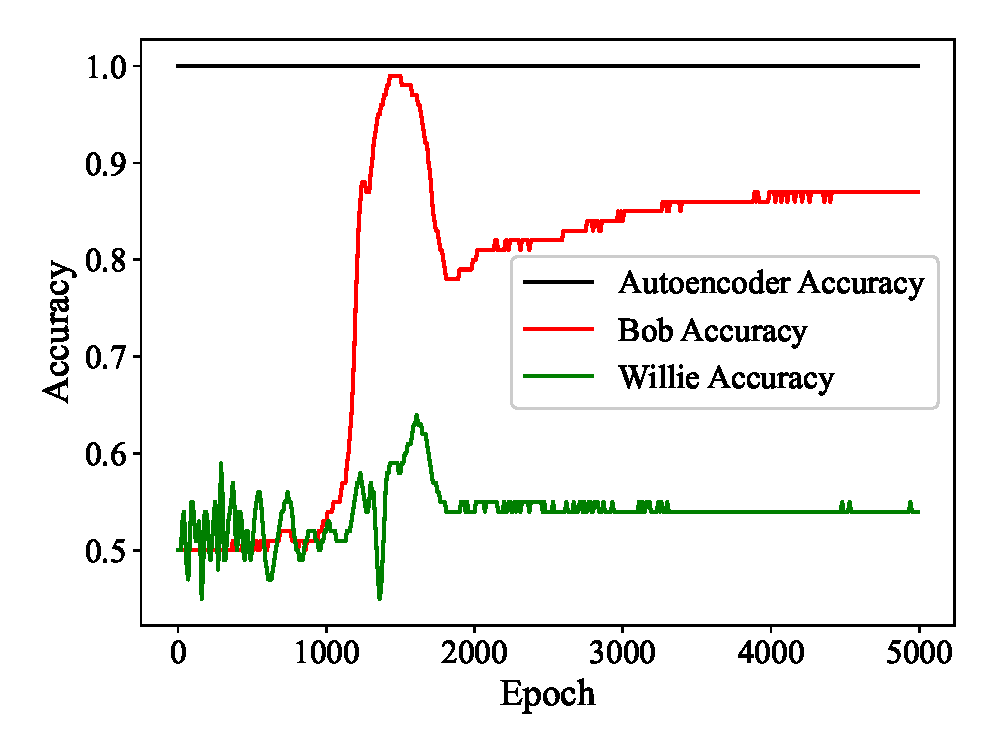
\includegraphics[width=\linewidth]{figs/multi_training_progress_awgn}
		\caption{AWGN channel}
	\end{subfigure}
	\hfill
	\begin{subfigure}{0.24\textwidth}
		\includegraphics[width=\linewidth]{figs/multi_training_progress_rayleigh}
		\caption{Rayleigh fading channel}	
	\end{subfigure}
	\caption{Evaluation results of our covert and autoencoder models during the training process show the system reaches a stable point after successful training.}
	\label{fig:multi_traning_progress}
\end{figure}


\textbf{Training Procedure}: In figure \ref{fig:traning_progress}, you can see the progress of each covert actor's accuracy on the test set during the training. It is evident from the plot that Bob gradually learns to decode covert messages \(m\) and establishes a working communication with Alice. Soon when the covert communication stabilizes, signals start to deviate from the distribution they had and this cause Willie to better tell them apart. When Willie's accuracy improves, the term \(\mathcal{L}_{Willie}\) dominates the other two objectives of Alice's loss function in (\ref{alice_loss}). Hence, Alice begins to gradually sacrifice its accuracy for covertness. These adjustments continue until the training process gets to a point where neither of the covert models improves no more. This will result in our models being successfully trained.


\textbf{Number of Users}: Figures \ref{fig:multi_awgn_results}, \ref{fig:multi_rayleigh_resutls} show our final model performances on two systems of 2-user and 4-user. It also demonstrates how numbers of users in the system affects our model's performance. Having more users in the system gives covert actors the ability to stay more covert. However, due to the system congestion, it will be more difficult for Alice and Bob to communicate reliably. More users' presence also causes heavier channel interference and consequently, we can see that covert users' impact on normal communications is slightly greater. Hence, it can be derived from the results that it becomes harder for covert models to establish a covert channel without impacting other users when there are already too many users in the system.


\textbf{Undetectibility}: In figures \ref{fig:multi_awgn_resutls_willie}, \ref{fig:multi_rayleigh_resutls_willie} we have visualized Willie's accuracy in percentage over a range of SNR values for classifying signals as normal and covert. These plots imply how probable it is for our covert signals to be detected by an observer at each SNR value. In both channel models, it is more probable for Willie to spot covert communication when there are fewer users in the system. We believe this is due to the more complex channel interference effect and noise model. When more users are communicating at the same time in the system, the distribution of channel effects becomes much more complex to learn for Willie.

\section{Conclusion}

\label{s:conc}


\bibliographystyle{IEEEtran}
\bibliography{bib/main}

\end{document}
